An heuristic is any approach to problem solving that employs a practical method that's not fully optimized but it's sufficient to reach an immediate short-term goal or approximation.\\
Given the NP-Hard nature of the Travelling Salesman Problem, finding the optimal solution may require a long time, hence the need to have heuristics method to find solutions that are close to the optimal.

\section{Nearest Neighbor}
A first approach to the TSP, is to consider the edges with the \textbf{smallest weights first} when choosing the next node in the cycle.\\
This type of logic is called \textbf{greedy}: a greedy algorithm chooses the locally optimal choice at each stage.

\begin{center}
    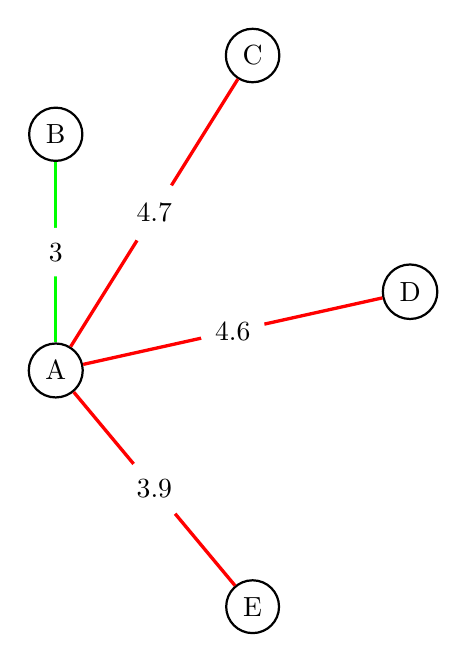
\begin{tikzpicture}
        \begin{scope}[every node/.style={circle,thick,draw}]
            \node (A) at (0,0) {A};
            \node (B) at (0,3) {B};
            \node (C) at (2.5,4) {C};
            \node (D) at (4.5,1) {D};
            \node (E) at (2.5,-3) {E};
        \end{scope}

        \begin{scope}[every node/.style={fill=white,circle},
                    every edge/.style={draw=red,very thick}]
            \path [-] (A) edge[draw=green] node {$3$} (B);
            \path [-] (A) edge node {$4.7$} (C);
            \path [-] (A) edge node {$4.6$} (D);
            \path [-] (A) edge node {$3.9$} (E);
        \end{scope}
    \end{tikzpicture}
\end{center}

In this example, among the edges connected to the node $A$, the edge $(A, B)$ is the one with the smallest weight, so node $B$ should be $A$'s successor.\\

By repeating this process for each new node added to the path and connecting the last node ($E$) to the starting node ($A$):

\begin{figure}[h]
    
    \centering
    \begin{subfigure}[c]{0.25\textwidth}
        \centering
        \resizebox{\linewidth}{!}{
            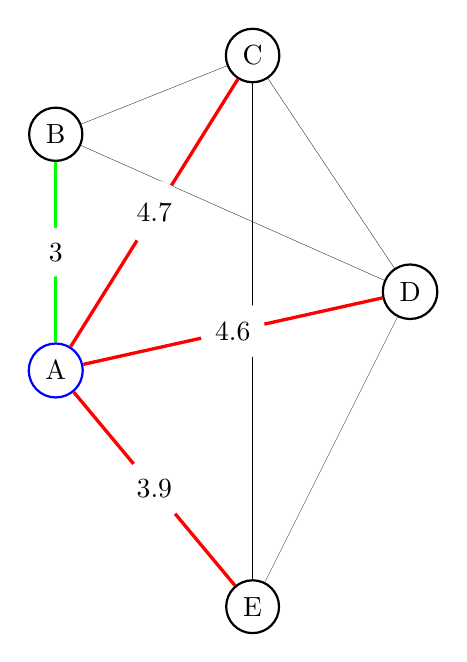
\begin{tikzpicture}
                \begin{scope}[every node/.style={circle,thick,draw}]
                    \node[draw=blue] (A) at (0,0) {A};
                    \node (B) at (0,3) {B};
                    \node (C) at (2.5,4) {C};
                    \node (D) at (4.5,1) {D};
                    \node (E) at (2.5,-3) {E};
                \end{scope}

                \begin{scope}[every node/.style={fill=white,circle},
                            every edge/.style={draw=red,very thick}]
                            \path [-] (B) edge[draw=black, ultra thin] (C);
                            \path [-] (B) edge[draw=black, ultra thin] (D);
                            \path [-] (C) edge[draw=black, ultra thin] (D);
                            \path [-] (C) edge[draw=black, ultra thin] (E);
                            \path [-] (D) edge[draw=black, ultra thin] (E);
                            \path [-] (A) edge[draw=green] node {$3$} (B);
                            \path [-] (A) edge node {$4.7$} (C);
                            \path [-] (A) edge node {$4.6$} (D);
                            \path [-] (A) edge node {$3.9$} (E);
                \end{scope}
            \end{tikzpicture}
        }
    \end{subfigure}$\Rightarrow$
    \begin{subfigure}[c]{0.25\textwidth}
        \centering
        \resizebox{\linewidth}{!}{
            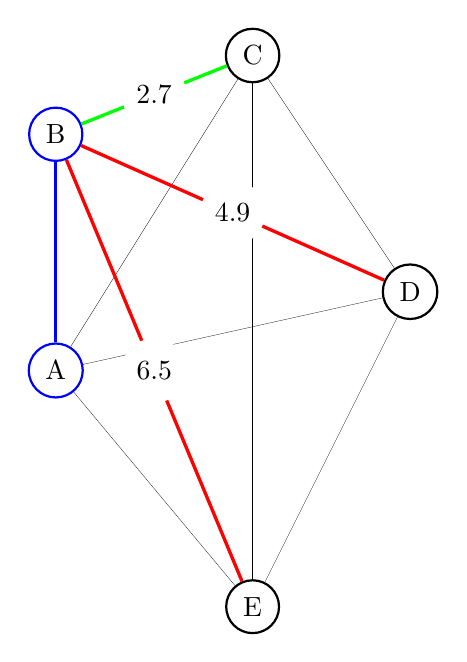
\begin{tikzpicture}
                \begin{scope}[every node/.style={circle,thick,draw}]
                    \node[draw=blue] (A) at (0,0) {A};
                    \node[draw=blue] (B) at (0,3) {B};
                    \node (C) at (2.5,4) {C};
                    \node (D) at (4.5,1) {D};
                    \node (E) at (2.5,-3) {E};
                \end{scope}

                \begin{scope}[every node/.style={fill=white,circle},
                            every edge/.style={draw=red,very thick}]
                    \path [-] (A) edge[draw=blue] (B);
                    \path [-] (C) edge[draw=black, ultra thin] (D);
                    \path [-] (D) edge[draw=black, ultra thin] (E);
                    \path [-] (E) edge[draw=black, ultra thin] (A);
                    \path [-] (A) edge[draw=black, ultra thin] (C);
                    \path [-] (A) edge[draw=black, ultra thin] (D);
                    \path [-] (C) edge[draw=black, ultra thin] (E);
                    \path [-] (B) edge[draw=green] node {$2.7$} (C);
                    \path [-] (B) edge[draw=red] node {$4.9$} (D);
                    \path [-] (B) edge[draw=red] node {$6.5$} (E);
                \end{scope}
            \end{tikzpicture}
        }
    \end{subfigure}$\Rightarrow$
    \begin{subfigure}[c]{0.25\textwidth}
        \centering
        \resizebox{\linewidth}{!}{
            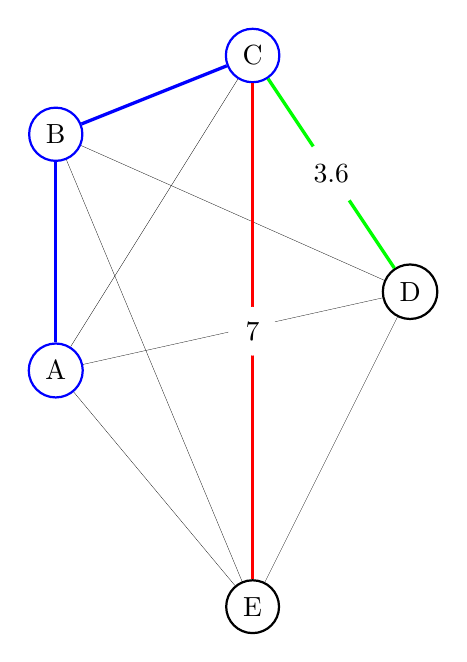
\begin{tikzpicture}
                \begin{scope}[every node/.style={circle,thick,draw}]
                    \node[draw=blue] (A) at (0,0) {A};
                    \node[draw=blue] (B) at (0,3) {B};
                    \node[draw=blue] (C) at (2.5,4) {C};
                    \node (D) at (4.5,1) {D};
                    \node (E) at (2.5,-3) {E};
                \end{scope}

                \begin{scope}[every node/.style={fill=white,circle},
                            every edge/.style={draw=red,very thick}]
                    \path [-] (A) edge[draw=blue] (B);
                    \path [-] (B) edge[draw=blue] (C);
                    \path [-] (C) edge[draw=green] node {$3.6$} (D);
                    \path [-] (D) edge[draw=black, ultra thin] (E);
                    \path [-] (E) edge[draw=black, ultra thin] (A);
                    \path [-] (A) edge[draw=black, ultra thin] (C);
                    \path [-] (A) edge[draw=black, ultra thin] (D);
                    \path [-] (B) edge[draw=black, ultra thin] (D);
                    \path [-] (B) edge[draw=black, ultra thin] (E);
                    \path [-] (C) edge[draw=red] node {$7$} (E);
                \end{scope}
            \end{tikzpicture}
        }
    \end{subfigure}$\Rightarrow$
    
\end{figure}
\begin{figure}[h]

    \centering$\Rightarrow$
    \begin{subfigure}[c]{0.25\textwidth}
        \centering
        \resizebox{\linewidth}{!}{
            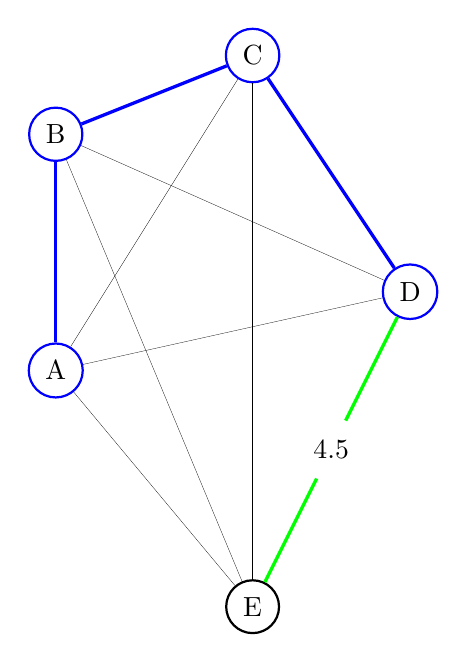
\begin{tikzpicture}
                \begin{scope}[every node/.style={circle,thick,draw}]
                    \node[draw=blue] (A) at (0,0) {A};
                    \node[draw=blue] (B) at (0,3) {B};
                    \node[draw=blue] (C) at (2.5,4) {C};
                    \node[draw=blue] (D) at (4.5,1) {D};
                    \node (E) at (2.5,-3) {E};
                \end{scope}

                \begin{scope}[every node/.style={fill=white,circle},
                            every edge/.style={draw=red,very thick}]
                    \path [-] (A) edge[draw=blue] (B);
                    \path [-] (B) edge[draw=blue] (C);
                    \path [-] (C) edge[draw=blue] (D);
                    \path [-] (E) edge[draw=black, ultra thin] (A);
                    \path [-] (A) edge[draw=black, ultra thin] (C);
                    \path [-] (A) edge[draw=black, ultra thin] (D);
                    \path [-] (B) edge[draw=black, ultra thin] (D);
                    \path [-] (B) edge[draw=black, ultra thin] (E);
                    \path [-] (C) edge[draw=black, ultra thin] (E);
                    \path [-] (D) edge[draw=green] node {$4.5$} (E);
                \end{scope}
            \end{tikzpicture}
        }
    \end{subfigure}$\Rightarrow$
    \begin{subfigure}[c]{0.25\textwidth}
        \centering
        \resizebox{\linewidth}{!}{
            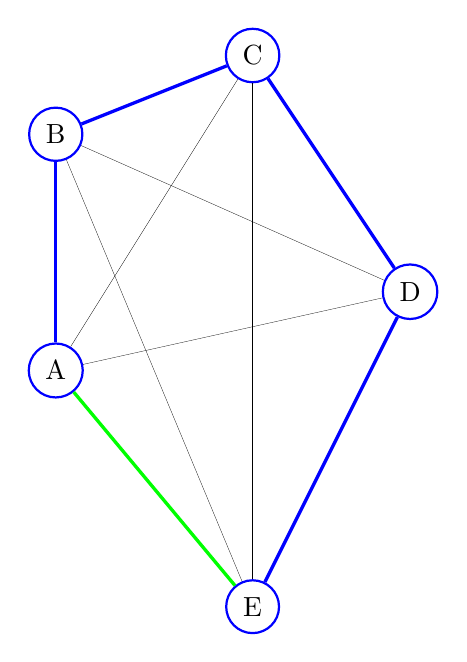
\begin{tikzpicture}
                \begin{scope}[every node/.style={circle,thick,draw}]
                    \node[draw=blue] (A) at (0,0) {A};
                    \node[draw=blue] (B) at (0,3) {B};
                    \node[draw=blue] (C) at (2.5,4) {C};
                    \node[draw=blue] (D) at (4.5,1) {D};
                    \node[draw=blue] (E) at (2.5,-3) {E};
                \end{scope}

                \begin{scope}[every node/.style={fill=white,circle},
                            every edge/.style={draw=red,very thick}]
                    \path [-] (A) edge[draw=blue] (B);
                    \path [-] (B) edge[draw=blue] (C);
                    \path [-] (C) edge[draw=blue] (D);
                    \path [-] (D) edge[draw=blue] (E);
                    \path [-] (E) edge[draw=green] (A);
                    \path [-] (A) edge[draw=black, ultra thin] (C);
                    \path [-] (A) edge[draw=black, ultra thin] (D);
                    \path [-] (B) edge[draw=black, ultra thin] (D);
                    \path [-] (B) edge[draw=black, ultra thin] (E);
                    \path [-] (C) edge[draw=black, ultra thin] (E);
                \end{scope}
            \end{tikzpicture}
        }
    \end{subfigure}$\Rightarrow$
    \begin{subfigure}[c]{0.25\textwidth}
        \centering
        \resizebox{\linewidth}{!}{
            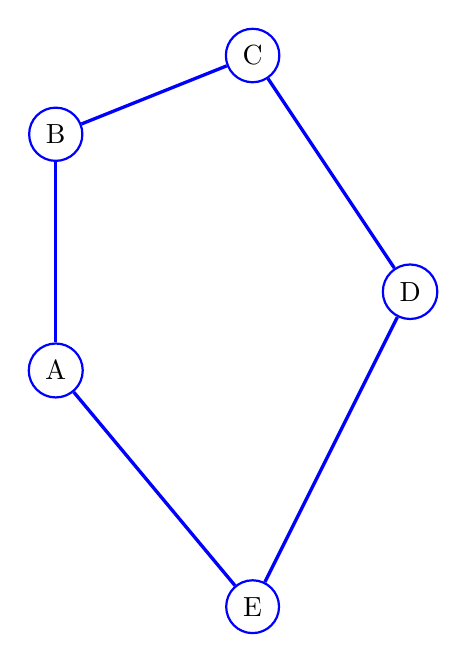
\begin{tikzpicture}
                \begin{scope}[every node/.style={circle,thick,draw}]
                    \node[draw=blue] (A) at (0,0) {A};
                    \node[draw=blue] (B) at (0,3) {B};
                    \node[draw=blue] (C) at (2.5,4) {C};
                    \node[draw=blue] (D) at (4.5,1) {D};
                    \node[draw=blue] (E) at (2.5,-3) {E};
                \end{scope}

                \begin{scope}[every node/.style={fill=white,circle},
                            every edge/.style={draw=red,very thick}]
                    \path [-] (A) edge[draw=blue] (B);
                    \path [-] (B) edge[draw=blue] (C);
                    \path [-] (C) edge[draw=blue] (D);
                    \path [-] (D) edge[draw=blue] (E);
                    \path [-] (E) edge[draw=blue] (A);
                \end{scope}
            \end{tikzpicture}
        }
    \end{subfigure}
    
\end{figure}

\subsection{Pseudocode}
\begin{algorithm}[h]
    \caption{Greedy algorithm for the TSP}
    \hspace*{\algorithmicindent} \textbf{Input} Starting node ($s\in V$), Set of nodes ($V$)\\
    \hspace*{\algorithmicindent} \textbf{Output} List of $n\coloneq|V|$ nodes forming an Hamiltonian cycle, Cost of the cycle
    \begin{algorithmic}

        \State $\mbox{cycle} \gets [s]$
        \State $\mbox{cost} \gets 0$
        
        \For{$i=0 \mbox{ to } n-2$}
            \State $\mbox{next} \gets \mbox{argmin}_{v}{\{c_{cycle[i], v}\;|\;v\in V\land v\not\in\mbox{cycle}\}}$
            \State $\mbox{cost}\gets\mbox{cost}+c_{cycle[i], next}$
            \State $\mbox{cycle}[i+1]\gets\mbox{next}$
        \EndFor
        \State $\mbox{cost}\gets\mbox{cost}+c_{cycle[n-1],s}$\\\\

        \Return cycle, cost
    \end{algorithmic}
\end{algorithm}
The solution found using the greedy algorithm is dependent to the starting node: a possible solution to this is to iterate through all possible starting nodes and keeping track of the best solution found so far.\\

\subsection{Results analysis}
\begin{figure}[h]
    \centering
    \includegraphics*[width=.6\textwidth]{1_1000_greedy_solution_plot.png}
    \caption*{Instance: \textbf{A}, Algorithm: \textbf{greedy}, Cost: \textbf{282030.8675}}
\end{figure}
The solutions found with the greedy algorithm are quite good, but sometimes the algorithm uses edges that cross a long distance, increasing a lot the cost of the solution.\\
This is caused by the fact that the greedy algorithm optimizes locally, without knowing wether that local choice is good or not in the long term: it might happen that after adding some edges to the cycle, the closest nodes are all already in the cycle, so the edge that will be considered may have a very large weight.\\
In the next section a tecnique is explored that will fix the problem of these edges.

\section{2-opt}
The 2-opt algorithm takes an existing cycle and tries to improve it's cost by changing some of the edges that compose the cycle without braking it.\\
The main idea behind the 2-opt algorithm is to find two edges that cross each other and fix them:

\begin{figure}[h]

    \centering
    \begin{subfigure}[c]{.4\textwidth}
        \centering
        \resizebox{\linewidth}{!}{
            \begin{tikzpicture}
                \begin{scope}[every node/.style={circle,thick,draw}]
                    \node (I) at (0,0) {$p_i$};
                    \node (JJ) at (0,3) {$p_{j+1}$};
                    \node (II) at (2.5,4) {$p_{i+1}$};
                    \node (J) at (4.5,1) {$p_j$};
                \end{scope}

                \begin{scope}[>={Stealth[black]}, every node/.style={fill=white,circle},
                            every edge/.style={draw=red,very thick}]
                    \path[->] (I) edge[draw=black] (II);
                    \path[->] (J) edge[draw=black] (JJ);
                    \path[->] (JJ) edge[dashed, draw=black, thin, bend right=90] (I);
                    \path[->] (II) edge[dashed, draw=black, thin, bend left=90] (J);
                \end{scope}
            \end{tikzpicture}
        }
    \end{subfigure}
    \raisebox{-0.5\height}{$\Rightarrow$}
    \begin{subfigure}[c]{.4\textwidth}
        \centering
        \resizebox{\linewidth}{!}{
            \begin{tikzpicture}
                \begin{scope}[every node/.style={circle,thick,draw}]
                    \node (I) at (0,0) {$p_i$};
                    \node (JJ) at (0,3) {$p_{j+1}$};
                    \node (II) at (2.5,4) {$p_{i+1}$};
                    \node (J) at (4.5,1) {$p_j$};
                \end{scope}

                \begin{scope}[>={Stealth[black]}, every node/.style={fill=white,circle},
                            every edge/.style={draw=red,very thick}]
                    \path[->] (I) edge[draw=blue] (J);
                    \path[->] (II) edge[draw=blue] (JJ);
                    %\path[-] (I) edge[dashed, draw=red, thin] (II);
                    %\path[-] (J) edge[dashed, draw=red, thin] (JJ);
                    \path[->] (JJ) edge[dashed, draw=black, thin, bend right=90] (I);
                    \path[->] (J) edge[dashed, draw=blue, bend right=90] (II);
                \end{scope}
            \end{tikzpicture}
        }
    \end{subfigure}
    \caption*{$p_i\coloneq\mbox{cycle}[i]$}

\end{figure}

This process is then repeated until any pair of edges that, if rearranged, lead to an improvement to the cost of the cycle, can't be found.\\
To find a pair of edges that can be changed to improve the cost it's sufficient to find a pair of nodes $p_i$, $p_j$, that satisfies the following inequality:
$$c_{p_i,p_{i+1}}+c_{p_j,p_{j+1}} > c_{p_i,p_{j}}+c_{p_{i+1},p_{j+1}}$$
Note that the cycle list is to be considered as a circular array: situations with indexes out of bounds or $i>j$ won't be treated in this paper since the fix is trivial.\\

If this inequality holds then swapping the edges $(p_i,p_j),\,(p_{i+1},p_{j+1})$ with $(p_i,p_{i+1}),$ $(p_{j},p_{j+1})$ will lower the cost of the cycle:
\begin{align*}
    \mbox{cost(new cycle)}&=\mbox{cost(old cycle)}-(c_{p_i,p_{i+1}}+c_{p_j,p_{j+1}})+(c_{p_i,p_{j}}+c_{p_{i+1},p_{j+1}})\\
    &\leq\mbox{cost(old cycle)}
\end{align*}

After finding the nodes $p_i$, $p_j$ the edges $(p_i, p_j)$ and $(p_{j+1}, p_{j+1})$ will take the place of the edges $(p_i, p_{i+1})$ and $(p_j, p_{j+1})$, reversing the route connecting $p_{i+1}\rightarrow p_{j}$.\\
Suppose the cycle is stored as a list of nodes ordered following the order of the nodes in the cycle, then this step can be done simply by \textbf{reversing the list} from the index $i+1$ to the index $j$:
$$[...,p_i,\underline{p_{i+1},...,p_j},p_{j+1},...]\Rightarrow[...,p_i,\underline{p_j,...(\mbox{reversed})...,p_{i+1}},p_{j+1},...]$$

\subsection{Pseudocode}
\begin{algorithm}
    \caption{2-opt algorithm for the TSP}
    \hspace*{\algorithmicindent}\hspace*{\algorithmicindent} \textbf{Input} List (cycle) of $n\coloneq|V|$ nodes forming an Hamiltonian cycle, Cost (cost) of the cycle\\
    \hspace*{\algorithmicindent} \textbf{Output} List of $n$ nodes forming an Hamiltonian cycle (with 2-opt swaps applied), Cost of the new cycle
    \begin{algorithmic}\\

        \While{*Exists a swap improving the cost*}
            \State $(i, j)\gets \mbox{find\_swap(cycle)}$
            \State $\mbox{cost}\gets\mbox{cost}-(c_{p_i,p_{i+1}}+c_{p_j,p_{j+1}})+(c_{p_i,p_{j}}+c_{p_{i+1},p_{j+1}})$
            \State $\mbox{reverse}(\mbox{cycle}, i+1, j)$
        \EndWhile\\\\

        \Return cycle, cost

    \end{algorithmic}
\end{algorithm}

\newpage

\subsection{Swap policy}
In this paper two different ways of finding a swap have been confronted:
\begin{enumerate}
    \item[-] Returning the \textbf{first swap} found that improves the cost
    \item[-] Looking among all possible pair of edges and returning the swap that improves the cost the most (the \textbf{best swap})
\end{enumerate}
Using the performance profiler it's easy to see that the best swap policy consistently finds better solutions than the first swap policy:
\begin{figure}[h]
    \centering
    \includegraphics*[width=.6\textwidth]{2opt_first_vs_best.png}
    \caption*{100 instances, Time limit: 120s}
\end{figure}
\newline
This is due to the fact that the first swap policy might get lost in improving the solution by a small amount by finding swaps in a region with an high concentration of nodes while the best swap policy aims to improve the edges with the highest weights.\\
This leads the best swap policy to fix immediatelly the worst edges, lowering right away the cost of the solution by a large amount.\\
It's also worth noticing that in application where the time limit is strict, the best swap policy is to be preferred since the big improvements will happen in the first iterations.

\subsection{Results analysis}
\begin{figure}[h]
    \centering
    \includegraphics*[width=.6\textwidth]{1_1000_g2opt-best_solution_plot.png}
    \caption*{Instance: \textbf{A}, Algorithm: \textbf{greedy+2opt (best swap)}, Cost: \textbf{244793.5477}}
\end{figure}
The 2opt algorithm is usually used after finding a cycle with the greedy algorithm to see wether it can be improved.\\
The solution displayed is obtained by running the 2opt algorithm, after applying the greedy algorithm on each possible starting node, and keeping the best one.\\

\newpage

Confronting this solution with the one showed for the greedy algorithm, it's possible to notice that the starting node used for the greedy algorithm has changed: even though the greedy algorithm found that starting node to be the best one (the one that generates the best cycle), after improving the solution using the 2opt algorithm, another starting node has been found to be better.\\
This is a phenomenon quite common in heuristics: when trying to improve two different solutions, improving the worse solution can lead to better results than improving the better one. This concept will be further explored in the metaheuristics chapter.

\section{Comparison Greedy / 2opt algorithms}
\begin{figure}[h]
    \centering
    \includegraphics*[width=.6\textwidth]{greedy_vs_g2opt.png}
    \caption*{100 instances, Time Limit: 120s}
\end{figure}

The 2opt algorithm manages to consistently improve the cost of the solutions of 15-20\% with respect to the solutions found by the greedy algorithm.